% !TeX program = xelatex
% !TeX encoding = UTF-8
% !TeX TXS-program:compile = txs:///xelatex | txs:///xelatex
\documentclass[aspectratio=169, table, 12pt]{beamer}
% Preamble bersama seluruh slide mata kuliah ini.
% Dipanggil dari slides/sessionXX/sessionXX.tex tepat sesudah baris
% \documentclass[aspectratio=169, table, 12pt]{beamer}
% Paket tambahan yang hanya dibutuhkan satu sesi ditulis di berkas sesi itu.

\usepackage{colortbl}
\usepackage{xcolor}
\usepackage{listings}
\usepackage{tabularx}
\usepackage{booktabs}
\usepackage{tikz}
\usepackage{pgfplots}
\pgfplotsset{compat=1.18}
\usetikzlibrary{arrows.meta, positioning, calc, fit, shapes.geometric,
	shapes.multipart, backgrounds, matrix, chains, trees}

\makeatletter
\def\input@path{{../theme/}}
\makeatother
\graphicspath{{../theme/}{../../figures/}}
\usetheme{Pradita}

\definecolor{praditagreen}{RGB}{37, 113, 71}

% Tema membuat garis tabel berwarna putih. Dikembalikan agar tabel terbaca.
\arrayrulecolor{black}
\setlength{\arrayrulewidth}{0.5pt}

\lstdefinelanguage{yaml}{
	basicstyle=\ttfamily\scriptsize,
	keywordstyle=\color{blue}\bfseries,
	commentstyle=\color{gray}\itshape,
	stringstyle=\color{red},
	showstringspaces=false,
	breaklines=true,
	frame=lines,
	numbers=none,
	backgroundcolor=\color{lightgray!10},
	tabsize=2,
	morecomment=[l]{\#}
}

\lstdefinelanguage{json}{
	basicstyle=\ttfamily\scriptsize,
	stringstyle=\color{red},
	commentstyle=\color{gray},
	breaklines=true,
	showstringspaces=false,
	tabsize=2,
	numbers=none,
	frame=lines,
	backgroundcolor=\color{lightgray!10},
	string=[s]{"}{"}
}

\lstdefinelanguage{bash}{
	keywords={},
	basicstyle=\ttfamily\scriptsize,
	ndkeywords={docker, kubectl, helm, curl, git, terraform},
	ndkeywordstyle=\color{purple}\bfseries,
	sensitive=true,
	commentstyle=\color{gray},
	numbers=none,
	breaklines=true,
	frame=lines,
	backgroundcolor=\color{lightgray!10},
	tabsize=2,
	comment=[l]{\#},
	showstringspaces=false
}

\lstdefinelanguage{http}{
	keywords={GET, POST, PUT, PATCH, DELETE, HEAD, OPTIONS, HTTP},
	basicstyle=\ttfamily\scriptsize,
	keywordstyle=\color{blue}\bfseries,
	sensitive=true,
	numbers=none,
	breaklines=true,
	frame=lines,
	backgroundcolor=\color{lightgray!10},
	tabsize=2,
	showstringspaces=false
}

\subtitle{IT40613 · Digital Platform \& API Economy}
\author{\textbf{Alfa Yohannis}}


\title{\Huge API untuk Agen AI\\ \vspace{10pt} dan Peta Jalan Platform}
\date{Pertemuan 14}

\begin{document}
\frame{\titlepage}

\begin{frame}
  \frametitle{Isi Pertemuan}
  \vspace{14pt}
  \begin{columns}[t]
    \column{0.5\textwidth}
    {\small\tableofcontents[sections={1-6}]}

    \column{0.5\textwidth}
    {\small\tableofcontents[sections={7-11}]}
  \end{columns}
\end{frame}

\begin{frame}{\hfill}
  \centering
  \Huge{\textbf{Agen memesan 60 janji.\\Kuota habis pada janji ke-38.\\Salah agen, atau salah API?}}
\end{frame}

\section{Tujuan dan Konteks}

\begin{frame}{{\Large Tujuan Pembelajaran}}
  \vspace{10pt}
  \begin{itemize}
    \item Menjelaskan cara agen AI memakai API dan peran MCP (\textit{Model Context Protocol}).
    \item Menilai kesiapan API organisasi untuk dipakai agen AI beserta risikonya.
    \item Menyusun peta jalan platform dan API yang merangkum tonggak C1 sampai C3.
  \end{itemize}
\end{frame}

\begin{frame}{{\Large Diagram Konsep Bab 14}}
  \centering
  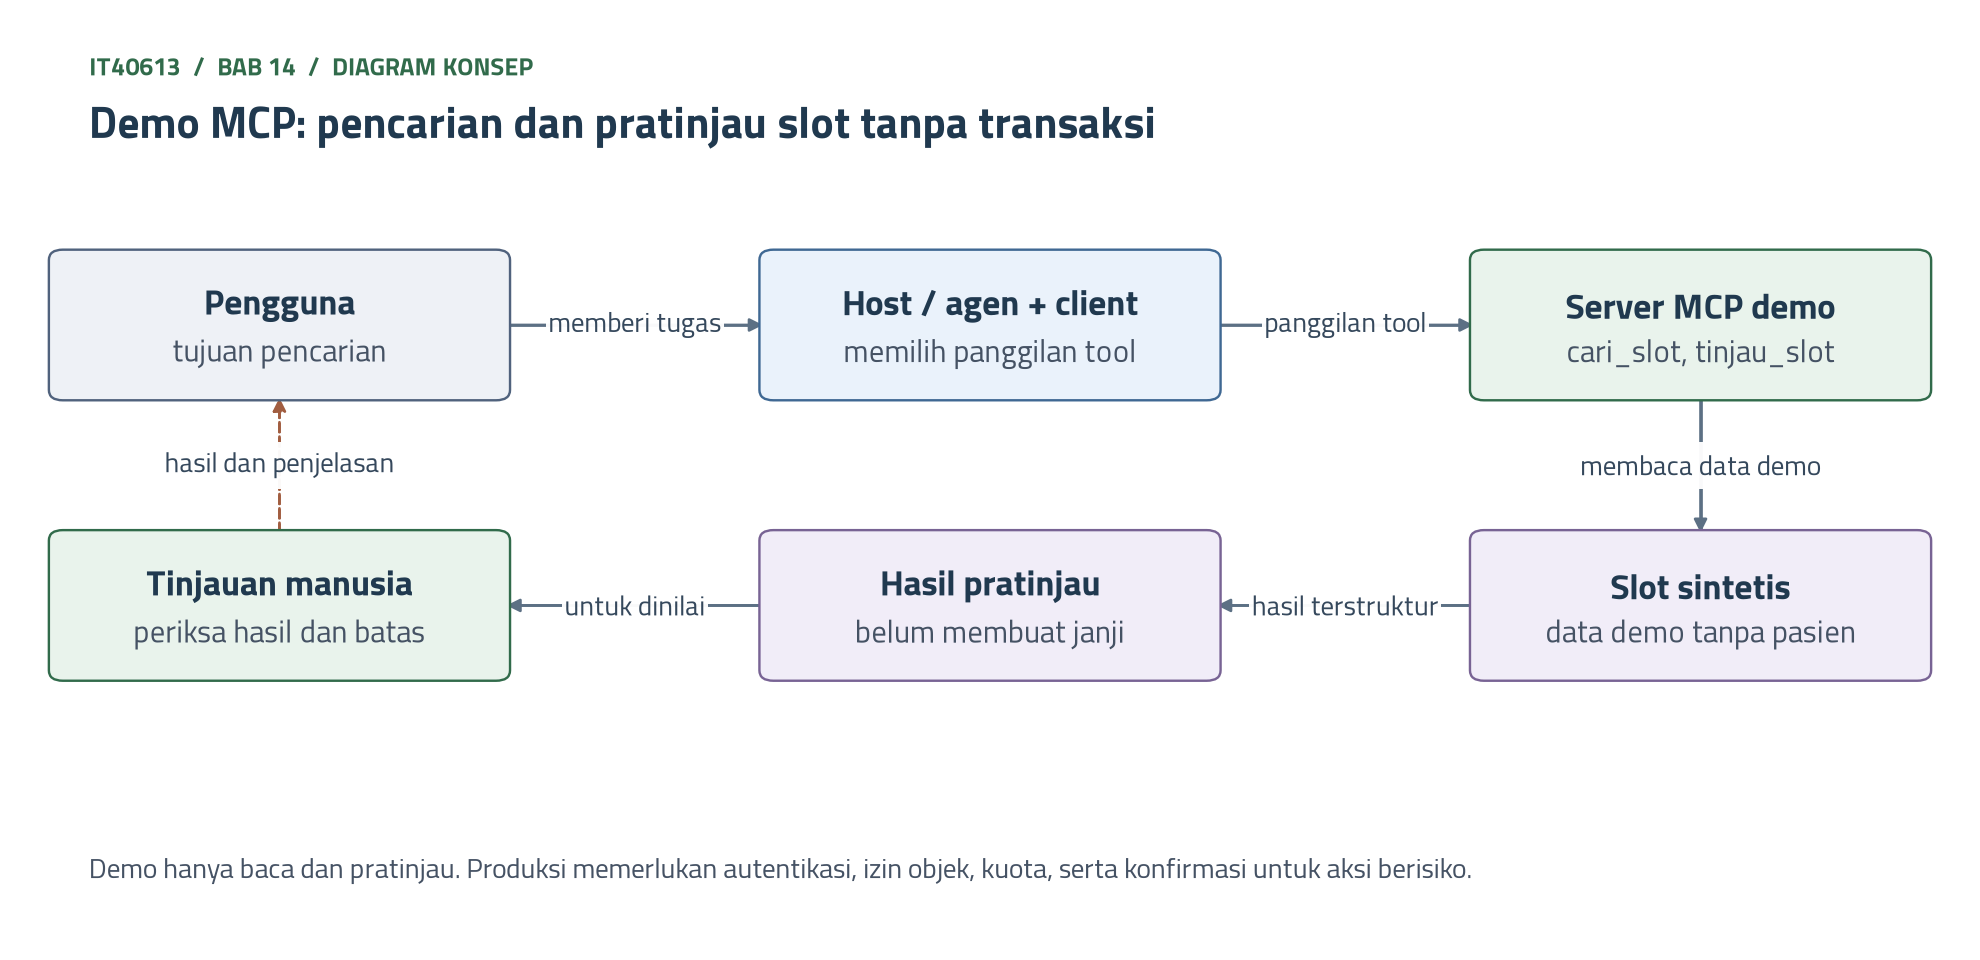
\includegraphics[width=0.96\textwidth,height=0.77\textheight,keepaspectratio]{../../figures/ch14-diagram-konsep.png}
\end{frame}

\section{Agen sebagai Pengguna API}

\begin{frame}{{\Large Agen AI sebagai Pengguna API}}
  \vspace{8pt}
  \begin{itemize}
    \item Agen memakai API untuk menyelesaikan tugas lewat serangkaian keputusan.
    \item Pilihan alat dipengaruhi konteks yang ditafsirkan model.
    \item Agen tetap tunduk pada kewenangan pengguna dan aturan bisnis server.
    \item Bila urutan panggilan dapat ditulis lebih dahulu, skrip biasa lebih murah.
    \item 36 rekap per bulan pada API-04 berurutan tetap, sehingga tidak perlu agen.
  \end{itemize}
  \vspace{6pt}
  {\small Analogi: asisten kantor boleh mencari jadwal, tetapi kewenangan menandatangani pesanan tetap dibatasi.}
\end{frame}

\begin{frame}{{\Large Pengembang Manusia dan Agen AI}}
  \footnotesize
  \begin{tabularx}{\textwidth}{>{\raggedright\arraybackslash}p{2.5cm} >{\raggedright\arraybackslash}X >{\raggedright\arraybackslash}X >{\raggedright\arraybackslash}X}
    \hline
    \textbf{Aspek} & \textbf{Pengembang} & \textbf{Agen AI} & \textbf{Akibat rancangan} \\ \hline
    Memahami kontrak & Saat membangun & Saat berjalan, tiap kali & Deskripsi ikut diuji \\ \hline
    Urutan panggilan & Tetap di dalam kode & Dipilih model & Batas langkah per tugas \\ \hline
    Galat & Dibaca saat pengujian & Dipakai untuk mencoba lagi & Sebut tindakan perbaikan \\ \hline
    Volume & 180 panggilan & 240 sampai 480 panggilan & Kuota per agen \\ \hline
    Tanggung jawab & Rilis, pengembang & Tugas, model, pihak diwakili & Audit menyimpan keduanya \\ \hline
  \end{tabularx}
\end{frame}

\begin{frame}{{\Large Dua Contoh Berangka}}
  \vspace{8pt}
  \begin{itemize}
    \item Medikara+: 3 panggilan per janji, 60 janji, 180 panggilan, kuota 300.
    \item Misalkan agen mencoba 3 tanggal di 2 rumah sakit: 8 panggilan per janji.
    \item Kebutuhan 480 panggilan: 37 janji selesai, 23 janji menerima kode 429.
    \item Misalkan 400 janji per bulan lewat agen, dan 2 persen salah pilih: 8 janji.
    \item Slot Rp250.000 ditambah telepon Rp15.000: Rp25,44 juta per tahun.
  \end{itemize}
\end{frame}

\section{Model Context Protocol}

\begin{frame}{{\Large Model Context Protocol}}
  \vspace{8pt}
  \begin{itemize}
    \item \textit{Host}, \textit{client}, dan server bertukar pesan JSON-RPC 2.0.
    \item Revisi 2026-07-28: permintaan mandiri, tanpa sesi tingkat protokol.
    \item Contoh dari revisi lama harus diperiksa sebelum dipakai.
    \item Proyek Agentic AI Foundation, Linux Foundation, sejak Desember 2025.
    \item Server MCP sebaiknya tipis. Aturan layanan tetap berada di API-01.
  \end{itemize}
  \vspace{6pt}
  {\small Analogi: soket adaptor menyamakan cara menghubungkan, tetapi fungsi dan izin perangkat tetap perlu dikenali.}
\end{frame}

\begin{frame}{{\Large Arsitektur MCP pada Perusahaan Klien}}
  \centering
  \eadiagram{../../figures/ch14-arsitektur-mcp.tex}
\end{frame}

\begin{frame}{{\Large Fitur MCP dan Batasnya}}
  \footnotesize
  \begin{tabularx}{\textwidth}{>{\raggedright\arraybackslash}p{2.0cm} >{\raggedright\arraybackslash}p{3.0cm} >{\raggedright\arraybackslash}X >{\raggedright\arraybackslash}X}
    \hline
    \textbf{Fitur} & \textbf{Dipakai oleh} & \textbf{Contoh} & \textbf{Batas} \\ \hline
    \textit{Tools} & Model, untuk dijalankan & \texttt{cari\_slot}, \texttt{tinjau\_slot} & Validasi, akses, batas laju \\ \hline
    \textit{Resources} & Pengguna atau model & Panduan tanpa data pasien & Bukan wewenang memesan \\ \hline
    \textit{Prompts} & Pengguna, sebagai templat & Permintaan jadwal & Tidak menambah izin \\ \hline
    \textit{Elicitation} & Server, lewat \textit{client} & Menanyakan pilihan slot & Jawaban tetap diperiksa \\ \hline
  \end{tabularx}

  \vspace{8pt}
  \small Anotasi \textit{tool} dianggap tidak tepercaya, kecuali berasal dari server tepercaya.
\end{frame}

\begin{frame}{{\Large Standar Tidak Otomatis Membayar Dirinya}}
  \vspace{8pt}
  \begin{itemize}
    \item 36 sambungan khusus: 36 $\times$ Rp45 juta, atau Rp1,62 miliar per tahun.
    \item Satu server MCP: satu antarmuka, Rp45 juta per tahun.
    \item Telepon berkurang: 3 menit, atau Rp3.000 per janji.
    \item Ambang: 15.000 janji per tahun, atau 1.250 per bulan.
    \item Satu perusahaan 400 janji per bulan hemat Rp14,4 juta: perlu sekitar 4.
  \end{itemize}
\end{frame}

\begin{frame}{{\Large Contoh Lokal: Cari dan Pratinjau}}
  \vspace{8pt}
  \begin{itemize}
    \item SDK resmi Python lini 2.x memakai \texttt{MCPServer}, diperiksa pada 2.3.0.
    \item \texttt{cari\_slot} membaca jadwal sintetis, \texttt{tinjau\_slot} menampilkan pratinjau.
    \item Demo tidak membuat pemesanan atau mengakses data pasien.
    \item Empat pemeriksaan lulus: cari, pratinjau, tolak fasilitas, tolak slot.
    \item Petunjuk: \berkas{sources/chapter14/contoh-server-mcp/README.md}.
  \end{itemize}
\end{frame}

\section{Protokol Agen Lainnya}

\begin{frame}{{\Large Protokol Agen Lainnya}}
  \vspace{8pt}
  \begin{itemize}
    \item A2A berfokus pada kerja sama antaragen, MCP pada agen dan alat.
    \item Konsep A2A: \textit{Agent Card}, \textit{Task}, \textit{Message}, \textit{Part}, \textit{Artifact}.
    \item Agen bekerja sama tanpa membuka keadaan internal atau alatnya.
    \item Misalkan 3 dari 36 perusahaan memakainya: Rp15 juta per perusahaan per tahun.
    \item Medikara menunda A2A. Pemicu: 12 dari 36 perusahaan memintanya.
  \end{itemize}
  \vspace{6pt}
  {\small Analogi: koordinasi antarpetugas berbeda dari cara satu petugas memakai perangkat kerjanya.}
\end{frame}

\begin{frame}{{\Large MCP, A2A, dan API Bisnis}}
  \centering
  \eadiagram{../../figures/ch14-mcp-a2a.tex}
\end{frame}

\section{Merancang API}

\begin{frame}{{\Large Merancang API yang Siap Dipakai Agen}}
  \vspace{8pt}
  \begin{itemize}
    \item Deskripsi tidak ambigu, \textit{schema} masukan, dan contoh hasil.
    \item Galat yang dapat ditindaklanjuti: 409 berarti minta pilihan baru.
    \item Baca, pratinjau, dan tulis dipisahkan agar persetujuan bermakna.
    \item Pratinjau memperlihatkan akibat. Konfirmasi menerima akibat itu.
    \item Nomor pratinjau bukan izin memesan. Server memeriksa kembali.
  \end{itemize}
  \vspace{6pt}
  {\small Analogi: formulir yang jelas memisahkan pencarian informasi, pemeriksaan isian, dan tanda tangan akhir.}
\end{frame}

\begin{frame}{{\Large Pemilahan Operasi API-01}}
  \footnotesize
  \begin{tabularx}{\textwidth}{>{\raggedright\arraybackslash}p{3.6cm} >{\raggedright\arraybackslash}p{1.6cm} >{\raggedright\arraybackslash}X}
    \hline
    \textbf{Operasi} & \textbf{Jenis} & \textbf{Syarat sebelum dibuka} \\ \hline
    \texttt{cariJadwalDokter} & Baca & Identitas agen, kuota, hasil sebagai data \\ \hline
    \texttt{pratinjauJanjiTemu} & Pratinjau & Hak atas karyawan, tanpa perubahan keadaan \\ \hline
    \texttt{bacaJanjiTemu} & Baca & Hanya janji milik pihak yang diwakili \\ \hline
    \texttt{buatJanjiTemu} & Tulis & Pratinjau, konfirmasi, kunci idempotensi \\ \hline
    \texttt{batalkanJanjiTemu} & Tulis & Konfirmasi, batas waktu pembatalan \\ \hline
    API-02 Hasil Pemeriksaan & Ditutup & Kontrak, penilaian dampak, keputusan forum \\ \hline
  \end{tabularx}

  \vspace{6pt}
  \small Operasi \texttt{pratinjauJanjiTemu} adalah usulan bab ini, belum ada pada kontrak 1.0.0.
\end{frame}

\begin{frame}{{\Large Peta Keputusan: Jalur Satu Aksi Agen}}
  \centering
  \eadiagram{../../figures/ch14-peta-keputusan.tex}
\end{frame}

\begin{frame}{{\Large Dua Perbaikan Berangka}}
  \vspace{8pt}
  \begin{itemize}
    \item Rentang tanggal dan satu pratinjau: 8 panggilan menjadi 4 per janji.
    \item Kebutuhan 480 turun menjadi 240, cadangan 60 dari kuota 300.
    \item Operasi baru masuk kelas B, membuka bagi agen masuk kelas C. Misalkan 80 jam.
    \item Misalkan 1 persen dari 400 janji terkirim dua kali: 4 janji ganda.
    \item Biayanya Rp12 juta per tahun. Kunci idempotensi 24 jam menutupnya.
  \end{itemize}
\end{frame}

\begin{frame}{{\Large Arazzo: Alur Bukan Bukti Aman}}
  \vspace{8pt}
  \begin{itemize}
    \item Arazzo mendefinisikan urutan panggilan dan ketergantungannya.
    \item Alur contoh: cari, pesan, baca status pada kontrak 1.0.0.
    \item Kode 409 mengarahkan alur kembali ke pencarian.
    \item Spesifikasi menyerahkan keamanan kepada pelaksana.
    \item Persetujuan manusia tidak tercatat, sehingga \textit{host} wajib berhenti.
  \end{itemize}
  \vspace{6pt}
  {\small Berkas: \berkas{sources/chapter14/alur-janji-temu.arazzo.yaml}. Pemeriksa: 3 langkah lulus, 0 temuan.}
\end{frame}

\section{Risiko dan Kendali}

\begin{frame}{{\Large Risiko dan Kendali}}
  \vspace{8pt}
  \begin{itemize}
    \item Aplikasi LLM mengaburkan batas antara data dan instruksi.
    \item OWASP: belum jelas ada pencegahan \textit{prompt injection} yang pasti.
    \item Kewenangan berlebih berakar pada fungsi, izin, atau otonomi.
    \item Otorisasi ditegakkan di sistem hilir, bukan diputuskan model.
    \item MCP tidak dapat menegakkan prinsip keamanannya pada tingkat protokol.
  \end{itemize}
  \vspace{6pt}
  {\small Analogi: instruksi pada kertas yang dibawa tamu tidak otomatis menjadi perintah sah bagi petugas.}
\end{frame}

\begin{frame}{{\Large Risiko, Kendali, dan Bukti Uji}}
  \scriptsize
  \begin{tabularx}{\textwidth}{>{\raggedright\arraybackslash}p{3.1cm} >{\raggedright\arraybackslash}X >{\raggedright\arraybackslash}X >{\raggedright\arraybackslash}p{3.0cm}}
    \hline
    \textbf{Risiko} & \textbf{Contoh Medikara} & \textbf{Kendali utama} & \textbf{Bukti uji} \\ \hline
    Instruksi tersembunyi (LLM01) & Keterangan jadwal berisi perintah & Kewenangan ditetapkan server & Skenario injeksi \\ \hline
    Kewenangan berlebih (LLM06) & Seluruh 4 operasi dibungkus & Buka sesedikit mungkin & Daftar \textit{tool} per peran \\ \hline
    Akses objek (API1) & Token sah membaca janji lain & Otorisasi tiap objek & Uji lintas objek \\ \hline
    Konsumsi (API4, LLM10) & 480 panggilan per hari & Kuota per agen, batas langkah & Uji pengulangan, 429 \\ \hline
    Data berlebih (LLM02) & Spesialis tujuan ke model & Minimalkan bidang & Tinjauan keluaran \\ \hline
    Janji ganda & Mengulang sesudah waktu habis & Kunci idempotensi & Uji kirim ulang \\ \hline
  \end{tabularx}

  \vspace{6pt}
  \small Kuota 100 per hari: 25 janji per hari. Batas 30 hari 3.000 panggilan, bukan 9.000.
\end{frame}

\begin{frame}{{\Large Kapan Manusia Ikut Memutuskan?}}
  \footnotesize
  \begin{tabularx}{\textwidth}{>{\raggedright\arraybackslash}p{3.6cm} >{\raggedright\arraybackslash}X >{\raggedright\arraybackslash}X}
    \hline
    \textbf{Kelas fungsi} & \textbf{Contoh pemesanan} & \textbf{Otomasi usulan} \\ \hline
    Mengambil informasi & Mencari slot dalam kuota & Tinggi: berjalan sendiri \\ \hline
    Menganalisis informasi & Membandingkan dengan jam kerja & Tinggi: alasan dapat diperiksa \\ \hline
    Memilih keputusan & Mengusulkan satu sampai tiga slot & Sedang: karyawan memilih \\ \hline
    Melaksanakan tindakan & Membuat atau membatalkan janji & Rendah: sesudah konfirmasi \\ \hline
  \end{tabularx}

  \vspace{8pt}
  \small Empat kelas fungsi mengikuti Parasuraman dkk. Pilihan tingkatnya adalah usulan latihan.

  \vspace{4pt}
  \small UU PDP Pasal 10: hak keberatan atas keputusan yang hanya didasarkan pada pemrosesan otomatis.
\end{frame}

\begin{frame}{{\Large Konfirmasi yang Masih Bermakna}}
  \vspace{8pt}
  \begin{itemize}
    \item Tinjauan 1 menit pada 400 janji: Rp4,8 juta per tahun.
    \item Bandingkan: salah pilih Rp25,44 juta, janji ganda Rp12 juta.
    \item Konfirmasi tiap panggilan: 3.200 per bulan, atau 13,33 jam.
    \item Rasa terlalu percaya tidak hilang hanya dengan latihan.
    \item Hanya aksi tulis: 400 konfirmasi, turun 87,5 persen.
  \end{itemize}
\end{frame}

\begin{frame}{{\Large Kasus Medikara: Uji Instruksi Tersembunyi}}
  \vspace{6pt}
  \begin{itemize}
    \item Misalkan 40 skenario di \textit{sandbox}, 20 berisi instruksi tersembunyi.
    \item Agen mengikuti 3 dari 20, atau 15 persen. Ketiganya ditolak dengan 403.
    \item Kesimpulan: model bukan kendali, kendali server bekerja pada skenario diuji.
    \item Keputusan: keterangan terstruktur, uji regresi, tiga penolakan menghentikan tugas.
    \item Harga: risiko sisa dicatat, bukan dinyatakan tertutup.
  \end{itemize}
\end{frame}

\section{Menilai Kesiapan}

\begin{frame}{{\Large Menilai Kesiapan Dua Operasi}}
  \footnotesize
  \begin{tabularx}{\textwidth}{>{\raggedright\arraybackslash}p{2.6cm} >{\raggedright\arraybackslash}p{1.4cm} >{\raggedright\arraybackslash}p{1.4cm} >{\raggedright\arraybackslash}X}
    \hline
    \textbf{Aspek} & \textbf{Cari} & \textbf{Buat} & \textbf{Bukti saat ini} \\ \hline
    Deskripsi & 1 & 1 & Kontrak ada, belum diuji pada agen \\ \hline
    Identitas & 1 & 1 & Rancangan API-06, tanpa identitas agen \\ \hline
    Otorisasi & 1 & 1 & Uji lintas objek belum ada \\ \hline
    Pratinjau & 2 & 0 & Operasi pratinjau belum ada \\ \hline
    Pengulangan & 2 & 1 & Kunci idempotensi belum diuji pada agen \\ \hline
    Konsumsi & 1 & 1 & Kuota per agen belum ada \\ \hline
    Konteks asing & 0 & 0 & Uji instruksi tersembunyi belum ada \\ \hline
    Audit & 1 & 1 & Catatan akses tanpa kolom agen \\ \hline
    \textbf{Jumlah} & \textbf{9} & \textbf{6} & Dari 16. Keduanya belum boleh dibuka \\ \hline
  \end{tabularx}
\end{frame}

\begin{frame}{{\Large Skor Tidak Dapat Menutup Syarat}}
  \vspace{8pt}
  \begin{itemize}
    \item Aksi baca: identitas, konsumsi, konteks asing, dan audit bernilai 2.
    \item Aksi tulis: seluruh delapan aspek bernilai 2.
    \item Skor 12 dengan pratinjau 0 tetap tertutup.
    \item Siap secara teknis berbeda dari layak secara bisnis: ambang 1.250 janji.
    \item Misalkan lapisan agen 480 jam: Rp28,8 juta, ditambah Rp45 juta per tahun.
  \end{itemize}
  \vspace{6pt}
  {\small Analogi: rem yang tidak berfungsi tidak dapat ditutup oleh pendingin udara dan cat baru.}
\end{frame}

\section{Merangkum Keputusan}

\begin{frame}{{\Large Telusur Keputusan: Bab 2 sampai 7}}
  \scriptsize
  \begin{tabularx}{\textwidth}{>{\raggedright\arraybackslash}p{1.0cm} >{\raggedright\arraybackslash}X >{\raggedright\arraybackslash}X}
    \hline
    \textbf{Bab} & \textbf{Keputusan yang dibawa} & \textbf{Akibat pada peta jalan} \\ \hline
    2 & Pasien Rp0, klinik masa uji enam bulan lalu Rp3 juta & Pendapatan sesudah masa uji \\ \hline
    3 & Uji lima klinik enam bulan, wasit merangkap pemain & Lima klinik lebih dulu \\ \hline
    4 & 20 sambungan, Rp45 juta per antarmuka, pagu Rp300 juta & Ukuran tiap antarmuka baru \\ \hline
    5 & Titik masalah INT-03, INT-02, INT-06 & API-01, KI-01 dan KI-02, API-02 \\ \hline
    6 & Token sah bukan izin, insiden 1.240 rekam & API-06 lebih dulu \\ \hline
    7 & Kesenjangan KI-01 sampai KI-08 & Kewajiban 600 jam di awal \\ \hline
  \end{tabularx}
\end{frame}

\begin{frame}{{\Large Telusur Keputusan: Bab 8 sampai 13}}
  \scriptsize
  \begin{tabularx}{\textwidth}{>{\raggedright\arraybackslash}p{1.0cm} >{\raggedright\arraybackslash}X >{\raggedright\arraybackslash}X}
    \hline
    \textbf{Bab} & \textbf{Keputusan yang dibawa} & \textbf{Akibat pada peta jalan} \\ \hline
    8 & API-06, API-01, API-02, sisanya antrean atau dirapikan & Isi gelombang, 7.680 jam \\ \hline
    9 & Kontrak API-01 1.0.0: 4 operasi, kunci idempotensi & Dasar \textit{tool} agen \\ \hline
    10 & Alternatif A bersyarat, masa transisi 6 bulan & Beban operasi 960 jam \\ \hline
    11 & Portal P2, SLA 99,0 persen, SLO 99,4 persen & Gerbang mitra \\ \hline
    12 & Paket berjenjang, impas lapisan 13 klinik & Sumbu waktu pendapatan \\ \hline
    13 & Federasi, kelas A sampai C, tanpa pemilik tanpa rilis & Perubahan urutan seperti kelas C \\ \hline
  \end{tabularx}

  \vspace{6pt}
  \small Kuota tetap 300 panggilan per hari per klinik, pada 40 klinik mitra, dengan tarif Rp60.000 per jam.
\end{frame}

\begin{frame}{{\Large Neraca Serentak: Satu Truk untuk Semua}}
  \footnotesize
  \begin{tabularx}{\textwidth}{>{\raggedright\arraybackslash}X >{\raggedright\arraybackslash}p{1.5cm} >{\raggedright\arraybackslash}p{1.5cm}}
    \hline
    \textbf{Pekerjaan pada 12 bulan yang sama} & \textbf{Jam} & \textbf{Sisa} \\ \hline
    KI-01, KI-02, API-06, API-01, API-02 (Bab 8), dari kapasitas 7.680 & 6.600 & 1.080 \\ \hline
    Operasi alternatif A (Bab 10) & 960 & 120 \\ \hline
    Pemeliharaan isi portal P2 (Bab 11) & 60 & 60 \\ \hline
    Federasi, bagian tim integrasi (Bab 13) & 227 & $-167$ \\ \hline
    Misalkan penyiapan A dan P2 oleh tim sendiri & 800 & $-967$ \\ \hline
    Uji coba \textit{gateway} (Bab 10), 5 klinik uji & 360 & $-1.327$ \\ \hline
  \end{tabularx}

  \vspace{8pt}
  \small Kekurangan 17,3 persen, setara Rp79,62 juta. Bab 13 sudah mencatat kurang 167 jam. Baris sesudahnya belum diuji pada bab sebelumnya.
\end{frame}

\section{Peta Jalan}

\begin{frame}{{\Large Menyusun Peta Jalan Platform dan API}}
  \vspace{8pt}
  \begin{itemize}
    \item Hasil layanan disusun dalam gelombang: nilai, prasyarat, kapasitas, gerbang.
    \item Peta jalan adalah pernyataan arah, bukan janji fitur pada tanggal tertentu.
    \item Kesiapan agen bukan alasan mendahulukan yang belum punya kontrak.
    \item IT40513: P8 (portal dan API mitra) tidak dirilis sebelum paket P2 dan P3 selesai. P8 berjalan Januari sampai Desember 2029, dan dibaca sebagai masa rilis mitra.
    \item Tanggal menyatakan kapan diperiksa, gerbang menyatakan bukti apa.
  \end{itemize}
  \vspace{6pt}
  {\small Analogi: membuka cabang dilakukan setelah pasokan, petugas, dan prosedur cabang awal terbukti berjalan.}
\end{frame}

\begin{frame}{{\Large Peta Jalan Tiga Gelombang}}
  \centering
  \eadiagram{../../figures/ch14-peta-jalan.tex}
\end{frame}

\begin{frame}{{\Large Hasil, Jam, dan Gerbang}}
  \scriptsize
  \begin{tabularx}{\textwidth}{>{\raggedright\arraybackslash}p{1.6cm} >{\raggedright\arraybackslash}X >{\raggedright\arraybackslash}p{2.2cm} >{\raggedright\arraybackslash}X}
    \hline
    \textbf{Gelombang} & \textbf{Hasil layanan} & \textbf{Jam} & \textbf{Gerbang keluar} \\ \hline
    1, 2027 & 5 klinik uji: jadwal nyata, pesan di \textit{sandbox}. KI-01, KI-02 tertutup & 7.007 dari 7.680, sisa 673 & Uji lintas objek 0 lolos, panggilan pertama 6,5 jam, tiket 1,08 \\ \hline
    2, 2028 & Medikara+ dan 18 klinik bertahap sejak April. API-02 Oktober. API-04 & 5.327 dari 7.680, sisa 2.353 & Salah gabung MPI di bawah 0,1 persen, SLO 99,4 persen selama 3 bulan \\ \hline
    3, 2029 sampai 2030 & 5 klinik Januari 2029, 35 klinik Juli 2029. Agen pada 2030 & 5.214 dari 15.360, sisa 10.146 & SLA 99,0 persen, 13 klinik membayar, delapan aspek bernilai 2 \\ \hline
  \end{tabularx}

  \vspace{8pt}
  \small Sisa 8,8 persen, 30,6 persen, lalu 66,1 persen. Rencana yang jauh ditulis sebagai arah, bukan janji.

  \vspace{4pt}
  \small Agen masih muat di Gelombang 1, sisa 193 jam. Penahannya prasyarat, bukan jam.
\end{frame}

\begin{frame}{{\Large Sumbu Waktu pada Titik Impas}}
  \vspace{8pt}
  \begin{itemize}
    \item 5 klinik membayar sejak Juli 2029, 35 klinik sejak Januari 2030.
    \item Pendapatan 2029 Rp90 juta, pendapatan 2030 Rp1,44 miliar.
    \item Sampai akhir 2029: biaya Rp896,4 juta, selisih Rp806,4 juta.
    \item Pada margin Rp919,2 juta, selisih tertutup sekitar 10,5 bulan kemudian.
    \item Kelonggaran 9 bulan pada P8: pendapatan dua tahun turun Rp1,08 miliar.
  \end{itemize}
  \vspace{6pt}
  {\small Hitungan kasar lapisan API-01. Biaya platform Rp2,4 miliar dihitung terpisah.}
\end{frame}

\begin{frame}{{\Large Yang Sengaja Ditunda}}
  \scriptsize
  \begin{tabularx}{\textwidth}{>{\raggedright\arraybackslash}p{3.7cm} >{\raggedright\arraybackslash}X >{\raggedright\arraybackslash}X}
    \hline
    \textbf{Inisiatif} & \textbf{Alasan} & \textbf{Pemicu peninjauan} \\ \hline
    Pemesanan agen tanpa konfirmasi & Otorisasi dan pengulangan belum teruji & 6 bulan aksi tulis dengan konfirmasi tanpa insiden \\ \hline
    A2A & Rp45 juta per tahun, pemakai sedikit & 12 dari 36 perusahaan memintanya \\ \hline
    API-03 Klaim Asuransi & 4.167 jam, manfaat Rp56,16 juta & Kontrak penjaminan Rp960 juta \\ \hline
    API-08 Resep Apotek & Belum ada pemilik & Jabatan pemilik ditunjuk \\ \hline
    Portal kustom P3 & Tidak sepadan pada 40 klinik & Lebih dari 100 organisasi \\ \hline
    \textit{Gateway} sendiri (B) & Kurang 2.760 jam & 2 staf terlatih, trafik dua kali lipat \\ \hline
  \end{tabularx}
\end{frame}

\begin{frame}{{\Large Kasus Medikara: Menggeser API-02}}
  \vspace{6pt}
  \begin{itemize}
    \item Digeser: rilis Oktober 2028, manfaat paling besar Rp104,4 juta tertunda.
    \item Dipertahankan: kontraktor Rp79,62 juta dan kerja ulang Rp30 juta.
    \item Selisih hanya Rp5,22 juta. Penentunya kas: tahun pertama sudah di atas pagu.
    \item Keputusan: 2.000 jam digeser, kelonggaran P8 perlu persetujuan keuangan.
    \item Agen ditahan sampai 2030, dengan gerbang bertahap.
  \end{itemize}
\end{frame}

\section{Aktivitas}

\begin{frame}{{\Large Aktivitas: Kesiapan Agen AI dan Peta Jalan}}
  \vspace{4pt}
  \begin{itemize}
    \item Bagian pertama: pilah operasi, nilai dua operasi, tetapkan aksi yang wajib disetujui.
    \item Bagian kedua: daftar keputusan, neraca jam dan uang, tiga gelombang, gerbang.
    \item Bisnis memimpin urutan nilai. Teknis memeriksa ketergantungan antar-API.
    \item Luaran C4: penilaian kesiapan, peta jalan, dan satu penundaan yang disengaja.
    \item Dipresentasikan menjelang UAS, menjadi masukan peta jalan IT40513.
  \end{itemize}
\end{frame}

\begin{frame}{{\Large Bacaan dan Lembar Kerja}}
  \vspace{8pt}
  \begin{itemize}
    \item \href{https://modelcontextprotocol.io/specification/2026-07-28}{Spesifikasi MCP 2026-07-28}
    \item \href{https://a2a-protocol.org/latest/specification/}{Spesifikasi A2A} dan \href{https://spec.openapis.org/arazzo/v1.1.0.html}{Arazzo 1.1.0}
    \item \href{https://genai.owasp.org/llm-top-10/}{OWASP Top 10 untuk aplikasi LLM 2025}
    \item \berkas{sources/chapter14/penilaian-kesiapan-agen-ai.md}
    \item \berkas{sources/chapter14/templat-peta-jalan-platform.md}
  \end{itemize}
\end{frame}

\section{Ringkasan dan Latihan}

\begin{frame}{{\Large Ringkasan}}
  \vspace{6pt}
  \begin{itemize}
    \item Agen memilih urutan saat berjalan, sehingga kuota dan deskripsi diuji lebih keras.
    \item MCP dan A2A tidak menggantikan kontrak, identitas, dan otorisasi API.
    \item Otorisasi ditegakkan di server. Manusia dilibatkan pada aksi tulis.
    \item Keputusan Bab 2 sampai 13 tidak muat pada 12 bulan: kurang 1.327 jam.
    \item Pesan utama: setiap pengguna baru masuk lewat kontrak, kewenangan, dan gerbang yang sama.
  \end{itemize}
\end{frame}

\begin{frame}{{\Large Latihan}}
  \vspace{6pt}
  \begin{enumerate}
    \item Jelaskan perbedaan API yang dirancang untuk pengembang manusia dengan API yang dipakai agen AI.
    \item Misalkan agen AI milik perusahaan klien ingin memesan jadwal dokter untuk karyawannya. Tentukan tiga batasan yang perlu diterapkan Medikara.
    \item Jelaskan alasan urutan gelombang dalam peta jalan tim, termasuk satu inisiatif yang sengaja ditunda.
  \end{enumerate}
\end{frame}

\end{document}
